\appendix{}
\appendixheaderon

\renewcommand{\loadeq}[1]{%
   \ExecuteMetaData[./equations/appendix.tex]{eq#1}%
}

\section{Schematic}
\label{app:schematic}
This section shows the schematic described in Section: \ref{sec:measCirc}.

\hypertarget{sch:TOC}{}
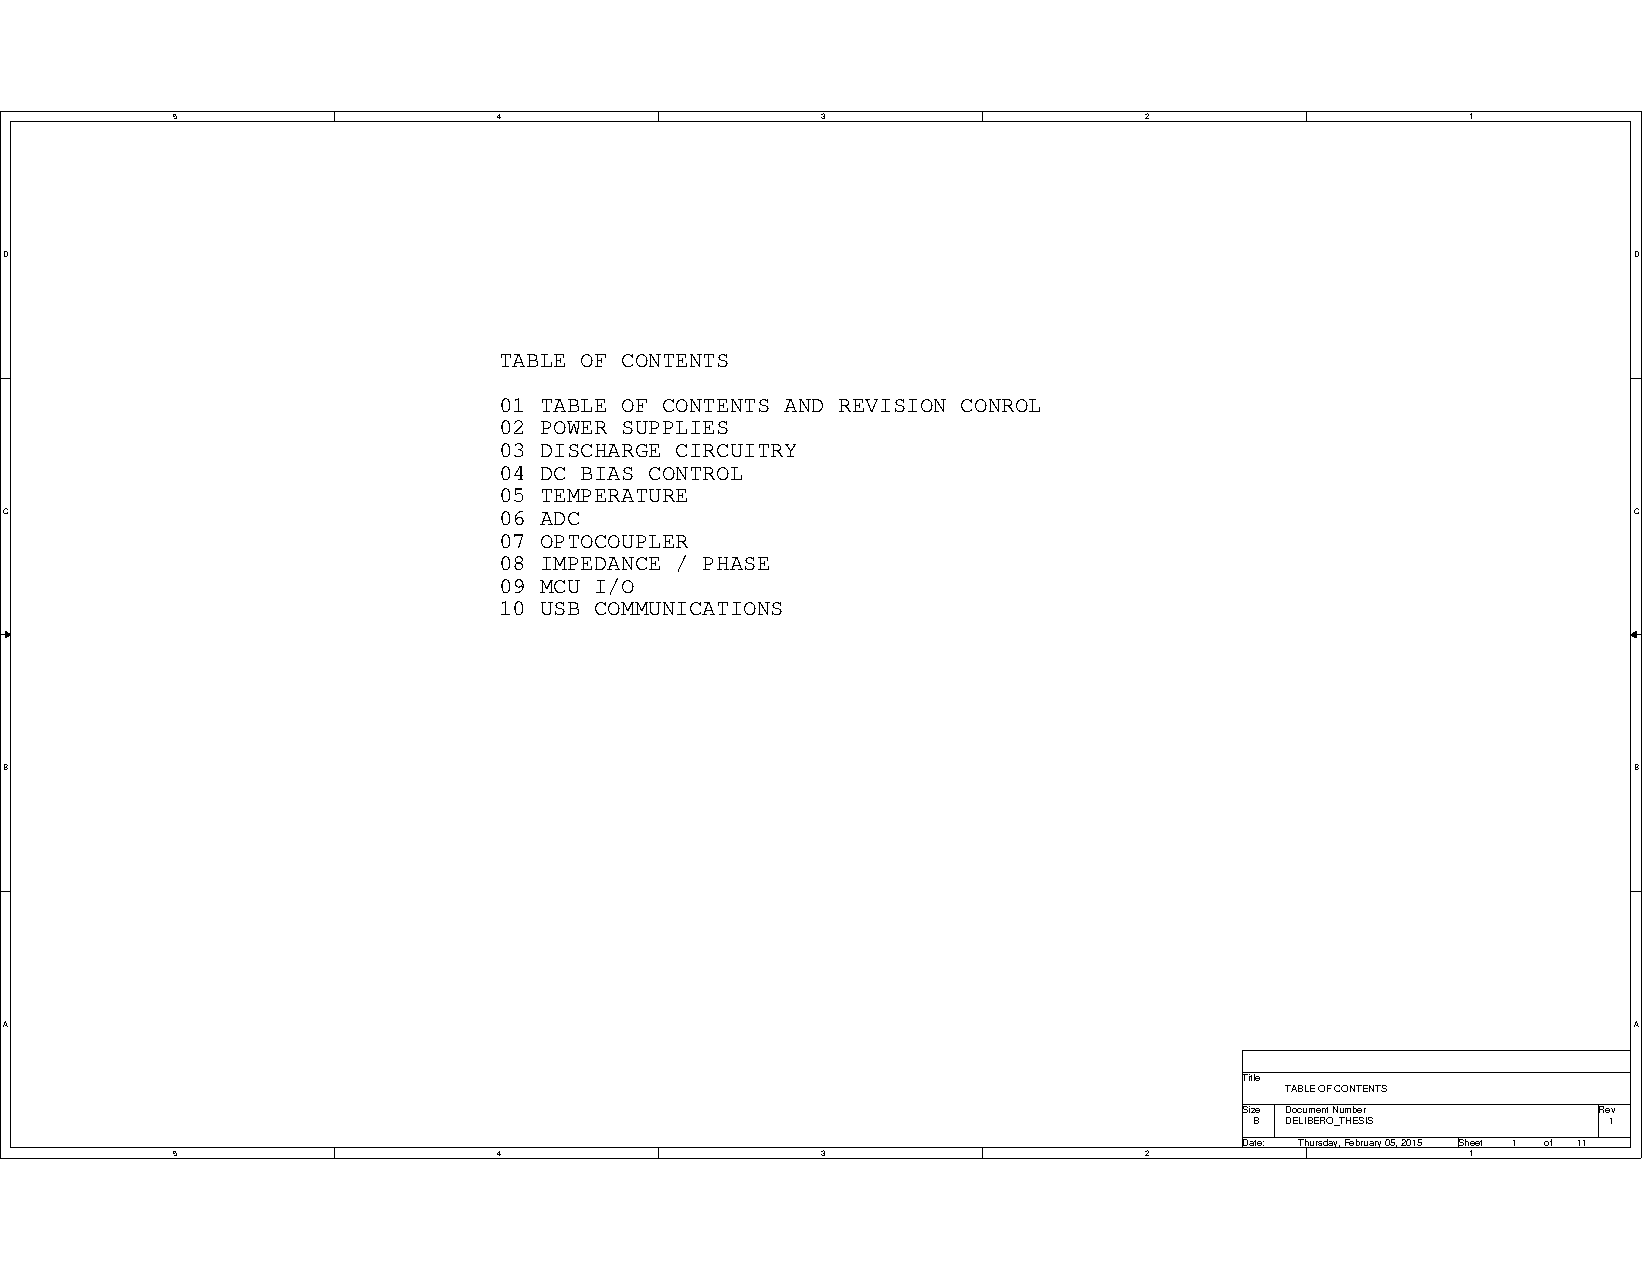
\includepdf[pages=1,angle=90,rotateoversize,offset=1.75in -.975in]{figures/board/capMeasCircuit.pdf}
\hypertarget{sch:Power}{}
\includepdf[pages=2,angle=90,rotateoversize,offset=1.75in -.975in]{figures/board/capMeasCircuit.pdf}
\hypertarget{sch:dcBias}{}
\includepdf[pages=3,angle=90,rotateoversize,offset=1.75in -.975in]{figures/board/capMeasCircuit.pdf}
\hypertarget{sch:opto}{}
\includepdf[pages=4,angle=90,rotateoversize,offset=1.75in -.975in]{figures/board/capMeasCircuit.pdf}
\hypertarget{sch:discharging}{}
\includepdf[pages=5,angle=90,rotateoversize,offset=1.75in -.975in]{figures/board/capMeasCircuit.pdf}
\hypertarget{sch:filtering}{}
\includepdf[pages=6,angle=90,rotateoversize,offset=1.75in -.975in]{figures/board/capMeasCircuit.pdf}
\hypertarget{sch:imph}{}
\includepdf[pages=7,angle=90,rotateoversize,offset=1.75in -.975in]{figures/board/capMeasCircuit.pdf}
\hypertarget{sch:adc}{}
\includepdf[pages=8,angle=90,rotateoversize,offset=1.75in -.975in]{figures/board/capMeasCircuit.pdf}
\hypertarget{sch:MCO I/O}{}
\includepdf[pages=9,angle=90,rotateoversize,offset=1.75in -.975in]{figures/board/capMeasCircuit.pdf}
\hypertarget{sch:Misc}{}
\includepdf[pages=10,angle=90,rotateoversize,offset=1.75in -.975in]{figures/board/capMeasCircuit.pdf}
\hypertarget{sch:com}{}
\includepdf[pages=11,angle=90,rotateoversize,offset=1.75in -.975in]{figures/board/capMeasCircuit.pdf}

\section{Generating Modeling Images}
\label{app:genModelingImages}
This appendix will list all of the matlab code and supporting files needed to generate the images seen in Section: \ref{sec:regression}.

\subsection{Example Data: Figure: \ref{fig:exCapData}}
\begin{figure}[ht!]
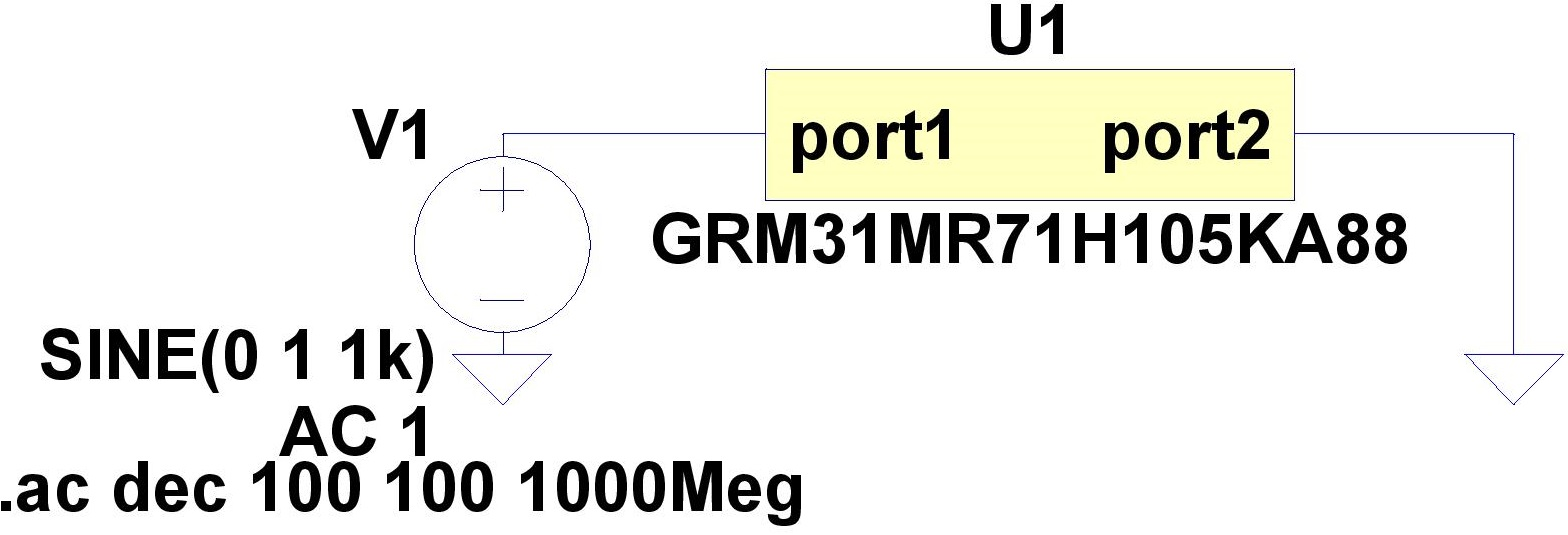
\includegraphics[keepaspectratio=true,width=2in]{./figures/appendix/exCapData_ltspice.jpg}
\centering
\caption{LTSpice Schematic for Capacitor Model}
\label{fig:exCapData_ltspice}
\end{figure}


This section will describe how to obtain and generate the example data used for the regression fitting. This method uses LTSpice to generate impedance vs frequency data from one of Murata's capacitor models. First, go to Murata's online SimSurfing tool \cite{simSurfing} and select the ``Monolithic Ceramic Capacitors'' button. Download a SPICE *.mod file (Appendix: \ref{app:subcir}) for the capacitor of interest, by selecting it from the list and clicking the ``netlist'' button. Open the *.mod file in LTSpice, right click on the part name in the line starting with ``.SUBCKT,'' and select ``Create Symbol.'' Create an LTSpice schematic similar to Figure: \ref{fig:exCapData_ltspice} and plot $\frac{V(n001)}{-I(V1)}$. The negative sign is important because LTSpice defines current as coming out of a node. If the negative sign is omitted, the phase will be offset by $180^o$, and the regression analysis will solve for negative capacitance! With the plot window selected, select  $``File\rightarrow Export\rightarrow Cartesian\rightarrow OK$'' with the impedance plot selected as the waveform. Open the resultant *.txt file, delete the first line, and change all tabs to commas (``$<:>\%s/<ctrl+v><TAB>/,/g$'' , ``$\%s/\string^I/,/g$'' in vim). Make sure to save the resultant file in ``/scripts/data.''

\subsubsection{Capacitor Subcircuit Model}
\label{app:subcir}
\lstinputlisting{./scripts/data/GRM31MR71H105KA88.mod}

\subsubsection{Plot ExCapData Script}
The functions used to get and plot the data can be found in Appendix: \ref{app:utilityFuns}.
\lstinputlisting{./scripts/regression/plot_ExCapData.m}

\subsection{Basic LSE Image: Figure: \ref{fig:basicLSE}}
\lstinputlisting{./scripts/regression/run_basicLSE.m}

\subsection{Levy's Method: Figures: \ref{fig:levy}, \ref{fig:levyIter_Err1}, \ref{fig:levyIter_Err2}, \& \ref{fig:levyIter}}
\lstinputlisting{./scripts/regression/run_levy_iter.m}
\lstinputlisting{./scripts/getInitGuess.m}
\lstinputlisting{./scripts/regression_levy_iter.m}

\subsection{Utility Functions}
\label{app:utilityFuns}
This appendix holds common ``utility'' functions used by many of the MATLAB scripts. You are required to manually save each plot after calling the ''plotfit.m.''

\lstinputlisting{./scripts/utilityFuns/getData.m}
\lstinputlisting{./scripts/utilityFuns/plotFit.m}
\lstinputlisting{./scripts/utilityFuns/plotType.m}


\section{Additional Regression Techniques}
\label{app:adtl_regression}
\nocite{neu_ModelSynth}
\nocite{cuth_regression}
\nocite{bbc_chebyshev}

% Run /scripts/appendix/powerSeries.m
\begin{figure}[ht!]
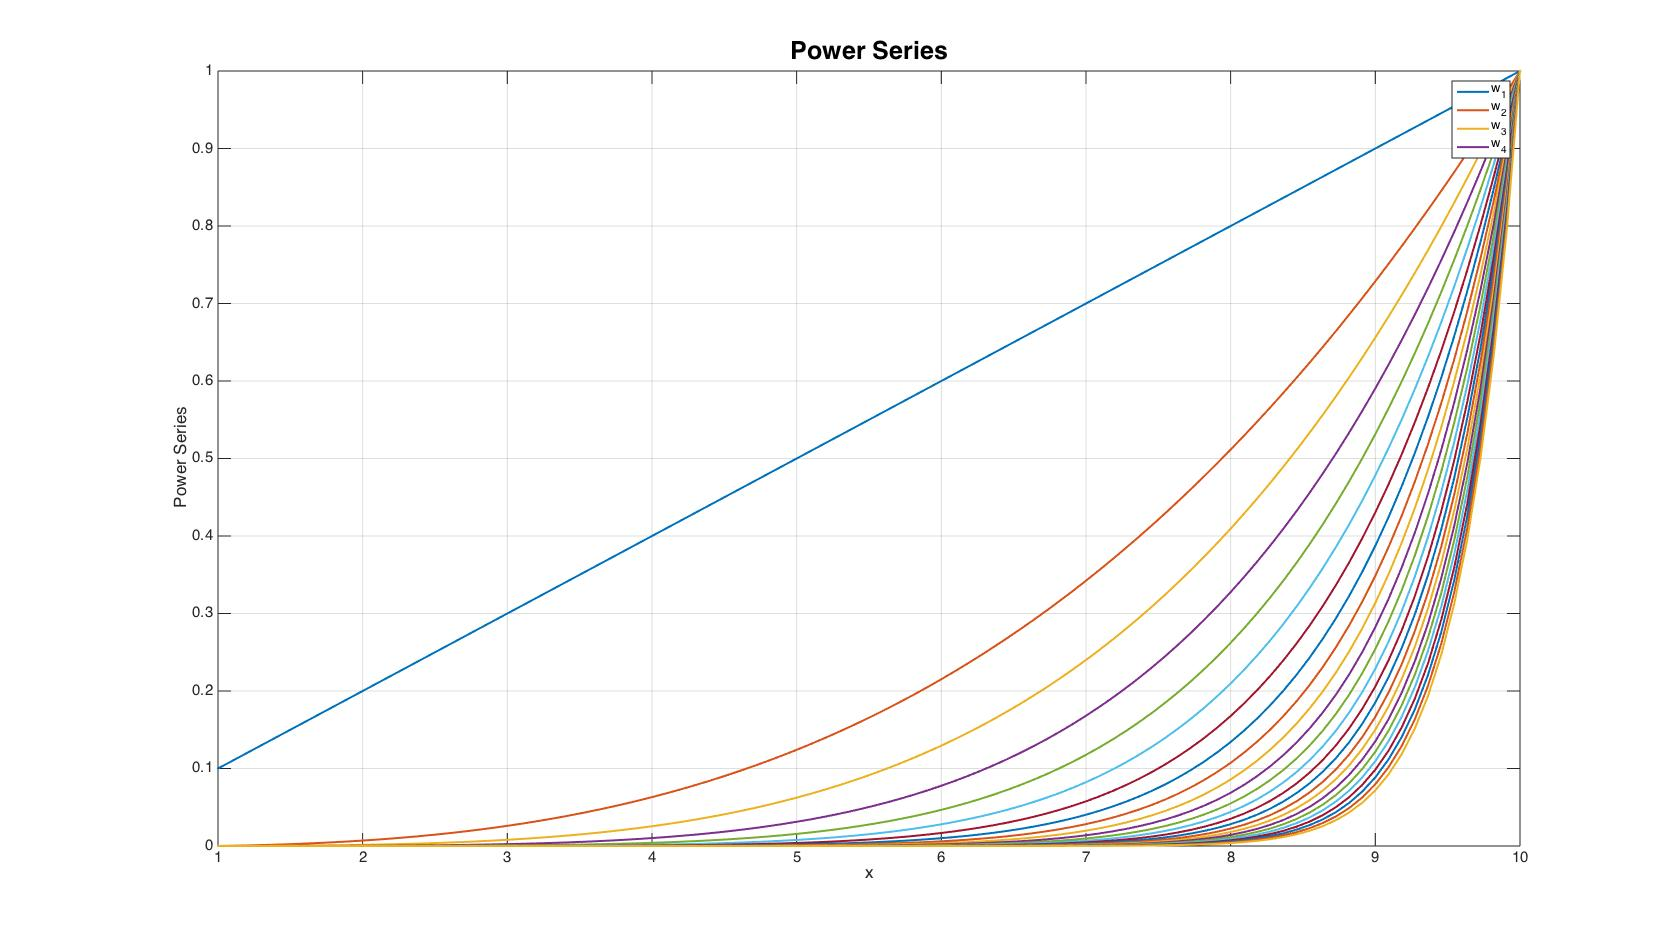
\includegraphics[keepaspectratio=true,width=6in]{./figures/appendix/powerSeries.jpg}
\centering
\caption{Power Series \cite{beyene_uwave}[Fig: 1]}
\label{fig:powerSeries}
\end{figure}



This section will cover the theory behind a computational method that should improve the results obtained in Section: \ref{sec:regression}. As previously stated, the main problem with applying Levy's approach to capacitor modeling is that it is ill-suited for wide bandwidth applications. As stated by Beyene, ``this is because the ordinary power series ${\omega ^0, \omega ^1, \omega ^2, \omega ^3,...}$ have a large dynamic range, and they become almost parallel at higher orders. As show in Figure: \ref{fig:powerSeries}, for higher orders, the shapes of the power series become very similar over most of the normalized frequency range. \cite{beyene_uwave}''

\begin{equation}
\label{equ:cheby}
T_{n+1} = 2xT_{n}-T_{n-1}
\end{equation}

\begin{equation}
    \label{equ:chebyPolys}
    \begin{split}
         T_0(x) &= 1           \\
         T_1(x) &= x           \\
         T_2(x) &= 2x^2-1      \\
         T_3(x) &= 4x^3-3x     \\
         T_4(x) &= 8x^4-8x^2+1 \\
         T_5(x) &= 16x^5-20x^3+5x
    \end{split}
\end{equation}

The proposed methodology uses Chebyshev polynomials of the first kind to circumvent this problem. As seen in Equation: \eqref{equ:cheby}, they are recursively defined with $T_0 = 1$ and $T_1 = x$. This results in polynomials that are orthogonal over a normalized frequency range, as seen in Figure: \ref{fig:cheby}. Gao\cite{gao_blackBox} shows that the frequency terms in an LSE can be replaced with Chebyshev polynomials. The coefficients found via this method are not the same as the coefficients in the frequency space. One needs to use Clenshaw's Recurrence Formula \cite{gao_blackBox}[Equation: 11] in order to get the desired coefficients. This method should produce a result that is more accurate due to its avoidance of the ill-conditioned matrix while solving the system of equations.

% Run /scripts/appendix/cheby.m
\begin{figure}[ht!]
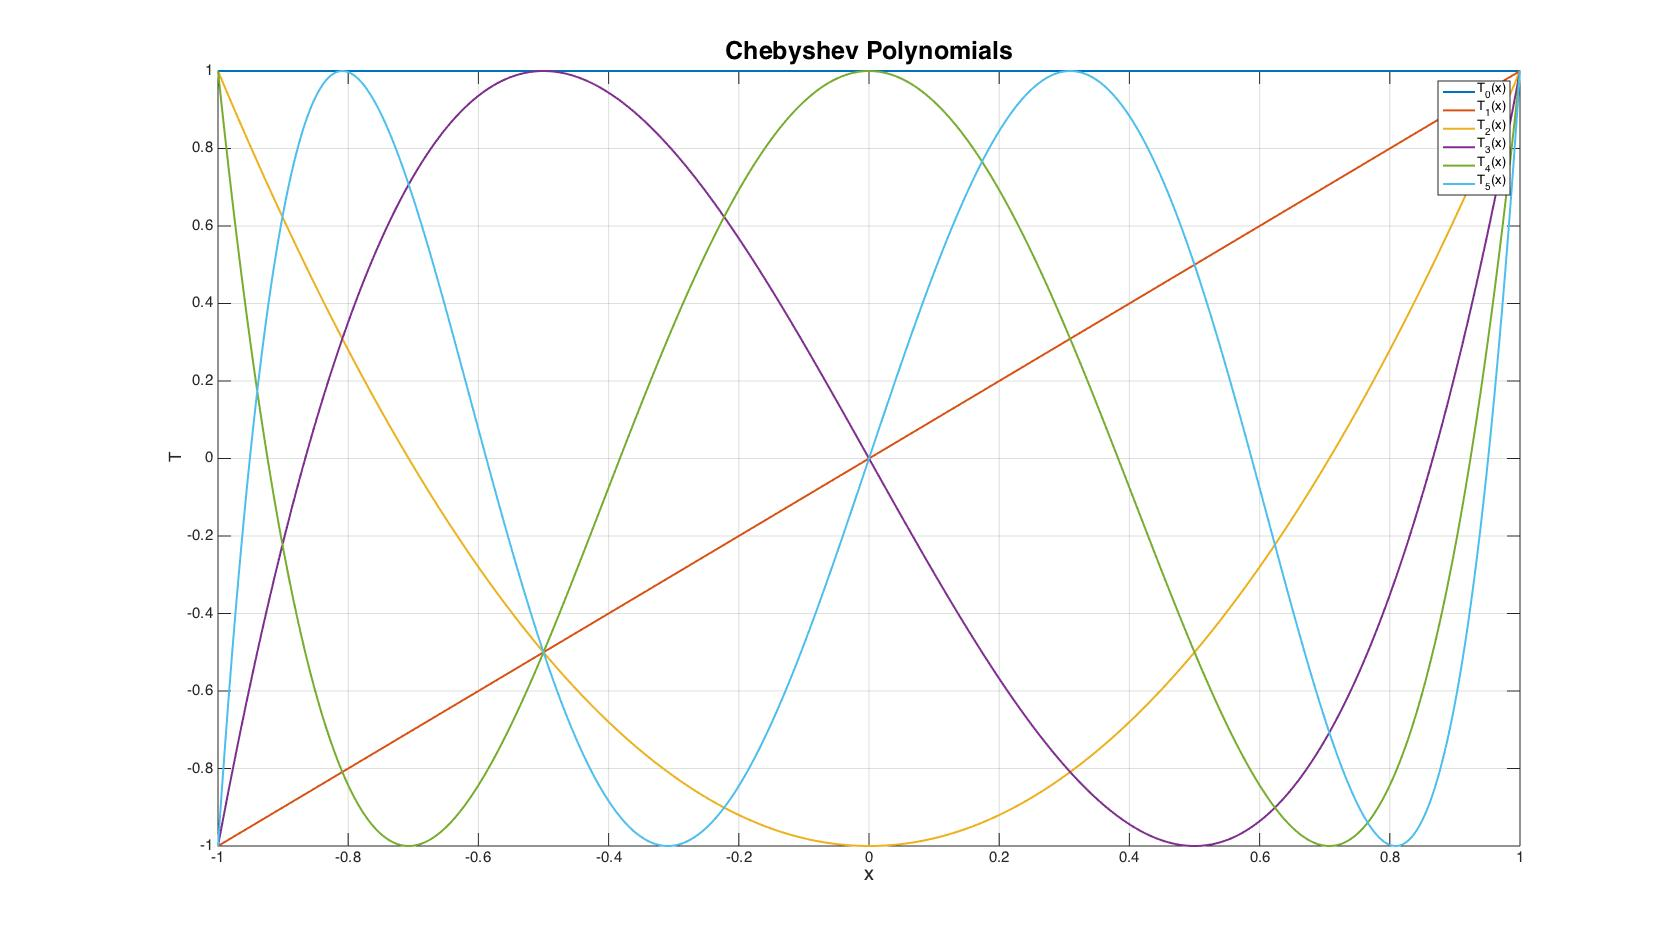
\includegraphics[keepaspectratio=true,width=6in]{./figures/appendix/cheby.jpg}
\centering
\caption{Chebyshev Polynomials \cite{wolf_cheby}}
\label{fig:cheby}
\end{figure}




\newpage
\section{Discharge Equations}
\label{app:disChargeEqs}
This section lists the discharge equations from Miller's electrochemical capacitor model \cite{electrochem_intro} seen in Figure: \ref{fig:superCap}.

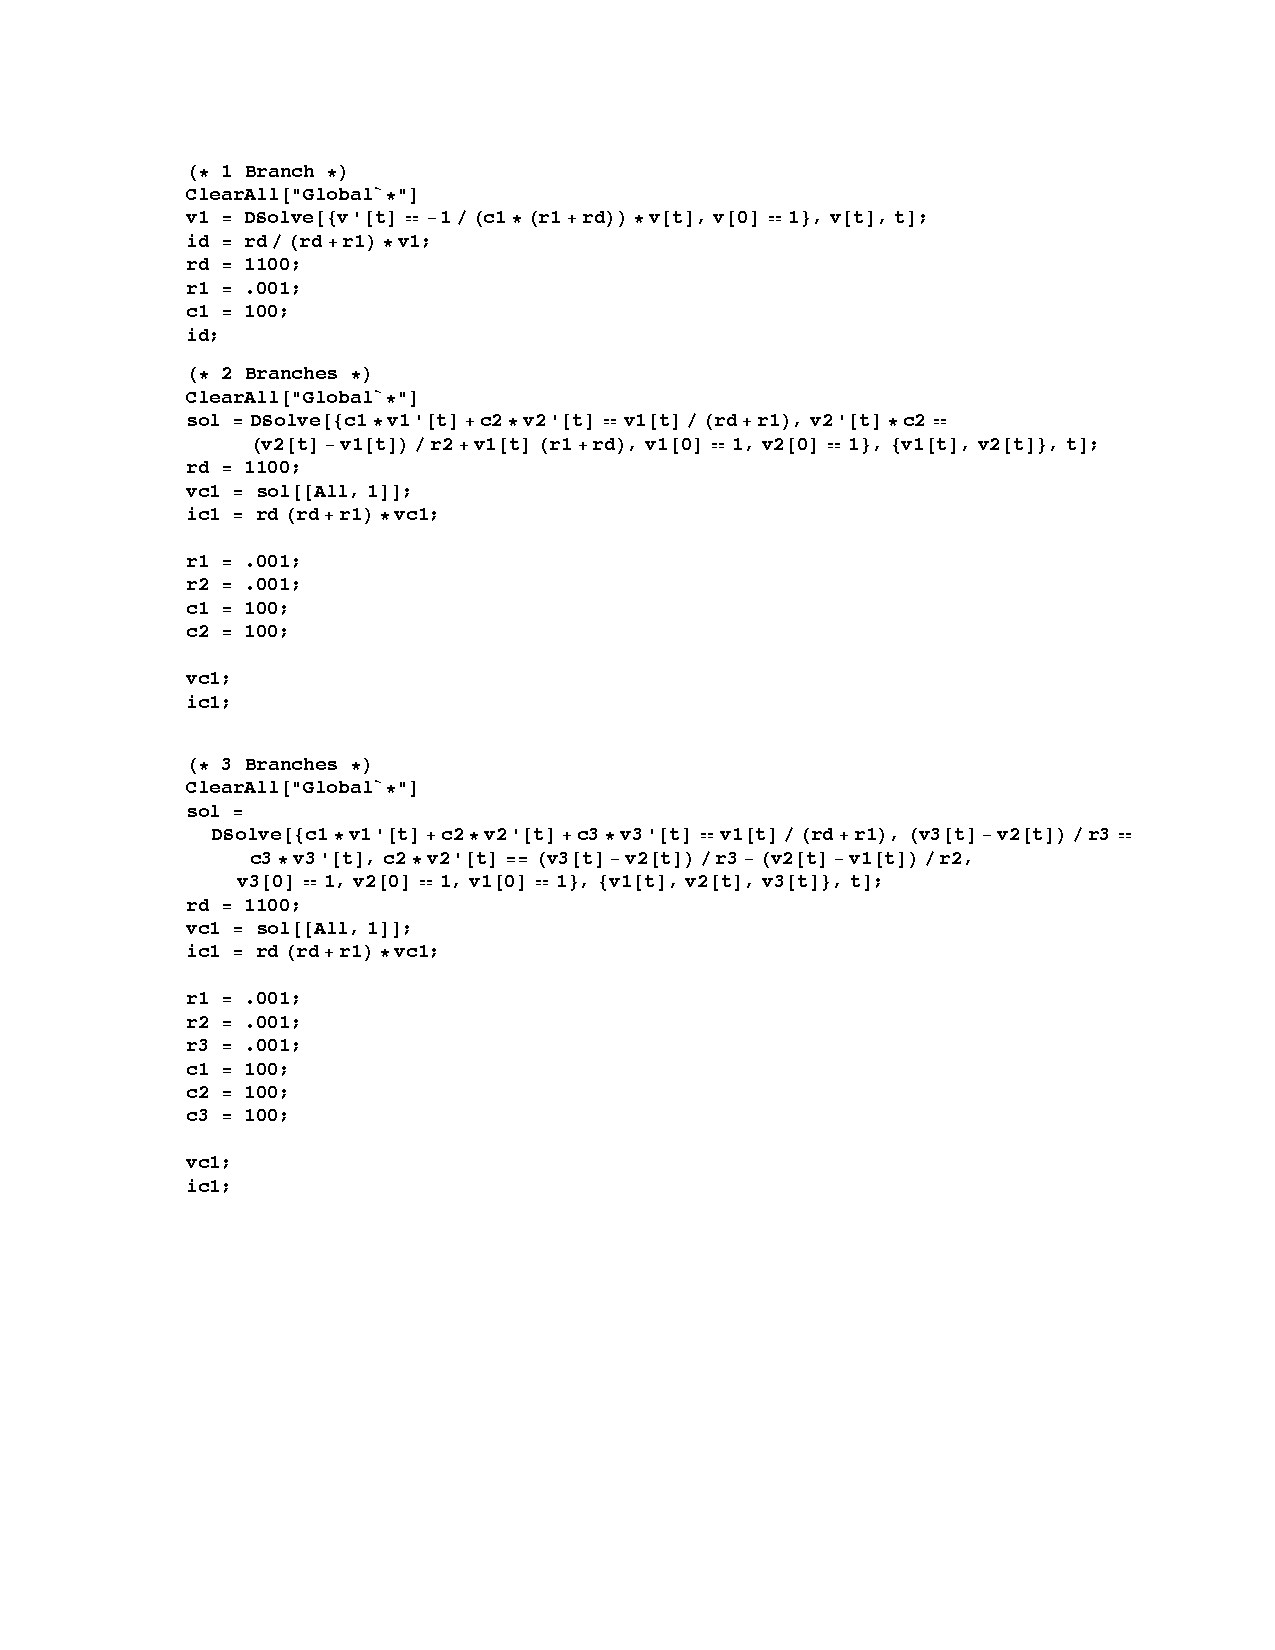
\includepdf[pages=-,offset=1.3in -1.3in,pagecommand={}]{scripts/discharge/discharge.pdf}


